\usetikzlibrary{shapes.geometric, arrows.meta, positioning, fit, shadows, shapes.symbols}

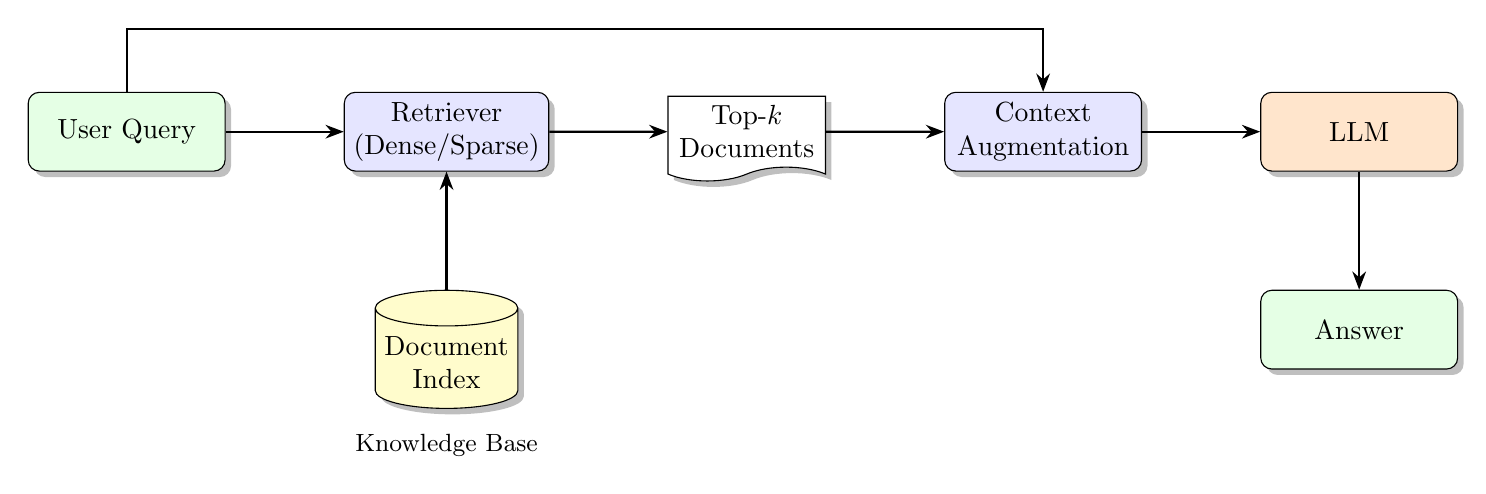
\begin{tikzpicture}[
    node distance=1.5cm,
    process/.style={
        draw,
        rectangle,
        rounded corners,
        minimum width=2.5cm,
        minimum height=1cm,
        align=center,
        fill=blue!10,
        drop shadow
    },
    database/.style={
        draw,
        cylinder,
        shape border rotate=90,
        aspect=0.25,
        minimum width=1.5cm,
        minimum height=1.5cm,
        align=center,
        fill=yellow!20,
        drop shadow
    },
    document/.style={
        draw,
        tape,
        tape bend top=none,
        minimum width=2cm,
        minimum height=1cm,
        align=center,
        fill=white,
        drop shadow
    },
    arrow/.style={
        ->,
        >=Stealth,
        thick
    }
]

% Nodes
\node[process, fill=green!10] (query) {User Query};
\node[process, right=of query] (retriever) {Retriever\\(Dense/Sparse)};
\node[database, below=of retriever] (index) {Document\\Index};
\node[document, right=of retriever] (docs) {Top-$k$\\Documents};
\node[process, right=of docs] (augment) {Context\\Augmentation};
\node[process, fill=orange!20, right=of augment] (llm) {LLM};
\node[process, fill=green!10, below=of llm] (answer) {Answer};

% Connections
\draw[arrow] (query) -- (retriever);
\draw[arrow] (retriever) -- (docs);
\draw[arrow] (index) -- (retriever);
\draw[arrow] (docs) -- (augment);
\draw[arrow] (augment) -- (llm);
\draw[arrow] (llm) -- (answer);

% Query also feeds into augmentation — route above intermediate nodes
\draw[arrow] (query.north) -- ++(0,0.8) -| (augment.north);

% Labels
\node[below=0.2cm of index, font=\small] {Knowledge Base};

\end{tikzpicture}
